% !TEX TS-program = Xelatex
% !TEX encoding = UTF-8 Unicode

% This is a simple template for a LaTeX document using the "article" class.
% See "book", "report", "letter" for other types of document.

\documentclass{article} % use larger type; default would be 10pt

%\usepackage[utf8]{inputenc} % set input encoding (not needed with XeLaTeX)
\usepackage{amsmath}
\usepackage{xeCJK} %调用 xeCJK 宏包
\setCJKmainfont{SimSun} %设置 CJK 主字体为 SimSun (宋体)
\setlength{\parindent}{44pt}
%%% Examples of Article customizations
% These packages are optional, depending whether you want the features they provide.
% See the LaTeX Companion or other references for full information.
\usepackage{figsize}
%%% PAGE DIMENSIONS
\usepackage{geometry} % to change the page dimensions
\geometry{a4paper} % or letterpaper (US) or a5paper or....
\geometry{margin=1in} % for example, change the margins to 2 inches all round
% \geometry{landscape} % set up the page for landscape
%   read geometry.pdf for detailed page layout information

\usepackage{graphicx} % support the \includegraphics command and options

% \usepackage[parfill]{parskip} % Activate to begin paragraphs with an empty line rather than an indent

%%% PACKAGES
\usepackage{amsmath}
\usepackage{booktabs} % for much better looking tables
\usepackage{array} % for better arrays (eg matrices) in maths
\usepackage{paralist} % very flexible & customisable lists (eg. enumerate/itemize, etc.)
\usepackage{verbatim} % adds environment for commenting out blocks of text & for better verbatim
\usepackage{subfig} % make it possible to include more than one captioned figure/table in a single float
% These packages are all incorporated in the memoir class to one degree or another...

%%% HEADERS & FOOTERS
\usepackage{fancyhdr} % This should be set AFTER setting up the page geometry
\pagestyle{fancy} % options: empty , plain , fancy
\renewcommand{\headrulewidth}{0pt} % customise the layout...
\lhead{}\chead{}\rhead{}
\lfoot{}\cfoot{\thepage}\rfoot{}

%%% SECTION TITLE APPEARANCE
\usepackage{sectsty}
\allsectionsfont{\sffamily\mdseries\upshape} % (See the fntguide.pdf for font help)
% (This matches ConTeXt defaults)

%%% ToC (table of contents) APPEARANCE
\usepackage[nottoc,notlof,notlot]{tocbibind} % Put the bibliography in the ToC
\usepackage[titles,subfigure]{tocloft} % Alter the style of the Table of Contents
\renewcommand{\cftsecfont}{\rmfamily\mdseries\upshape}
\renewcommand{\cftsecpagefont}{\rmfamily\mdseries\upshape} % No bold!
\renewcommand{\arraystretch}{1.5}
%%% END Article customizations


%%% The "real" document content comes below...

\title{预科实验一:测定冰的熔化热}
\author{朱寅杰 1600017721 周五12组}
\date{2017年9月29日} % Activate to display a given date or no date (if empty),
         % otherwise the current date is printed 

\begin{document}
\maketitle


\section{实验数据}
实验共计进行了四次,均使用电子天平(最小精度为0.01g)测量所涉及各物体的质量,使用铂电阻温度计实时测量实验过程中的量热器内的温度,并录像记录。

\paragraph{质量的测量:}
量热器内筒连同搅拌器的质量为$m_{cup}$=141.29g。各次实验中直接测量的量为开始时内筒搅拌器连同温水的质量$m_{cup+water}$,以及冰化完后内筒搅拌器连同凉水的质量$m_{cup+water+ice}$。从中计算出参与混合的温水质量$m_{water}$与冰的质量$m_{ice}$。\\
\begin{tabular*}{0.96\textwidth}{@{\extracolsep{\fill}}c|c c|c c}
\hline
序号&$m_{cup+water}$/g&$m_{cup+water+ice}$/g&$m_{water}$/g&$m_{ice}$/g\\
\hline
1&335.90&361.56&194.61&25.66\\
2&327.82&354.38&186.53&26.56\\
3&350.81&377.75&209.52&26.94\\
4&350.34&377.36&209.05&27.02\\
\hline
\end{tabular*}
\paragraph{冰的初温:}
各次实验时,冷库中冰的初温如下:\\
\begin{tabular*}{0.96\textwidth}{@{\extracolsep{\fill}}c|c c c c}
\hline
序号&1&2&3&4\\
\hline
$t_{ice}$&-23.9&-23.5&-23&-23.1\\
\hline
\end{tabular*}
\paragraph{熔化过程温度记录}
四次实验温度随时间变化的数据从录像中整理出记录在表中:\\
\begin{tabular*}{0.96\textwidth}{@{\extracolsep{\fill}}c c|c c|c c|c c}
\hline
第一次&&第二次&&第三次&&第四次&\\
时刻/s&温度/℃&时刻/s&温度/℃&时刻/s&温度/℃&时刻/s&温度/℃\\
\hline
0&38.0 &0&41.7 &0&34.2 &0&32.1 \\
32&37.9 &23&41.6 &40&34.1 &40&32.1 \\
55&37.8 &42&41.5 &47&33.8 &53&31.8 \\
70&37.7 &45&41.4 &51&33.7 &64&31.0 \\
73&37.2 &48&40.9 &57&33.5 &70&30.6 \\
76&36.0 &53&40.7 &63&32.6 &76&30.1 \\
80&35.8 &58&39.7 &69&31.7 &82&29.4 \\
103&35.1 &65&38.6 &75&30.8 &88&28.6 \\
108&33.3 &70&37.6 &81&30.3 &94&28.2 \\
111&32.3 &76&36.7 &87&30.0 &100&27.5 \\
117&31.1 &82&35.8 &93&29.3 &106&27.0 \\
121&30.1 &88&34.6 &99&28.7 &112&26.5 \\
126&28.9 &94&33.5 &105&28.3 &118&26.0 \\
131&28.0 &100&32.8 &111&28.0 &124&25.6 \\
136&27.2 &106&32.2 &117&27.5 &130&25.0 \\
142&26.6 &112&31.6 &123&27.1 &136&24.9 \\
148&26.2 &118&31.1 &129&26.8 &148&24.1 \\
154&25.9 &124&30.6 &135&26.4 &160&23.4 \\
160&25.2 &130&30.0 &141&26.1 &166&23.0 \\
166&25.3 &136&29.4 &147&25.9 &178&22.6 \\
172&25.2 &142&29.0 &153&25.6 &188&22.2 \\
178&25.1 &148&28.6 &159&25.3 &196&22.0 \\
184&25.0 &154&28.3 &165&25.0 &214&21.5 \\
190&24.8 &160&28.0 &171&24.9 &232&21.0 \\
196&24.7 &166&27.7 &177&24.6 &250&20.7 \\
202&24.6 &172&27.4 &189&24.1 &268&20.2 \\
208&24.5 &178&27.1 &201&23.8 &286&19.9 \\
214&24.4 &184&26.9 &219&23.3 &304&19.7 \\
226&24.3 &190&26.8 &237&22.9 &322&19.5 \\
238&24.2 &196&26.7 &255&22.6 &340&19.4 \\
262&24.1 &202&26.6 &267&22.3 &364&19.3 \\
286&24.2 &208&26.5 &285&22.0 &394&19.4 \\
304&24.2 &214&26.4 &303&21.6 &&\\
&&220&26.3 &321&21.4 &&\\
&&244&26.1 &333&21.3 &&\\
&&268&26.0 &345&21.2 &&\\
&&311&26.0 &369&21.1 &&\\
\hline
\end{tabular*}

\paragraph{投冰温度计算}
由于是录像记录,因此甚至无需使用外推法,只需在录像中读出投冰前一瞬间温度计的示数即可。\\
\begin{tabular*}{0.96\textwidth}{@{\extracolsep{\fill}}c|c c c c}
\hline
序号&1&2&3&4\\
\hline
投冰时间/s&69&41&39&50\\
投冰温度$t_{water}$/℃&37.8&41.6&34.2&32.1\\
\hline
\end{tabular*}
\paragraph{计算熔化热}
根据书上的公式\[L=(m_{cup}c_{Cu}+m_{water}c_{water})(t_{water}-t_{final})/m_{ice}-c_{water}t_{final}+c_{ice}t_{ice}\]
代入各数据,计算出四次实验的熔化热分别为3.20、3.39、3.23、3.18(单位:$10^5$J/K)
\section{讨论}
\paragraph{}
对比标准值3.34×$10^3$J/K,实验有三次偏小一次偏大。从公式中容易看出,对最终测得的L影响最大的量是冰的质量。实验进行中,只有第二次称量时在盖子上沾了些水没进杯子里,其他的几次实验均未有会损失冰的质量的情况。
\paragraph{}
实验中感受最明显的误差来源是冰从冷库中取出到投入量热器的过程中,即便隔着毛巾依然能透过寒意感受到我的手正在向冰大量传热。由于投冰的过程需要很小心,因此手上拿着冰的时间并不能无限制地短,导致冰投入时的温度比记录的冷库温度高不少。所记录的冰的温度每偏低1℃,熔化热的数值就会偏低0.02×$10^5$J/K。这样的误差还是相当可观的。
\paragraph{}
从下一页的图线上看冰熔化的全过程,可以明显的看出我在哪几秒钟搅拌的不够勤快。如果能将实验精度提高,兴许能做一个冰熔解时吸热速率的动力学分析。

\begin{figure}
\SetFigLayout{1}{1}
{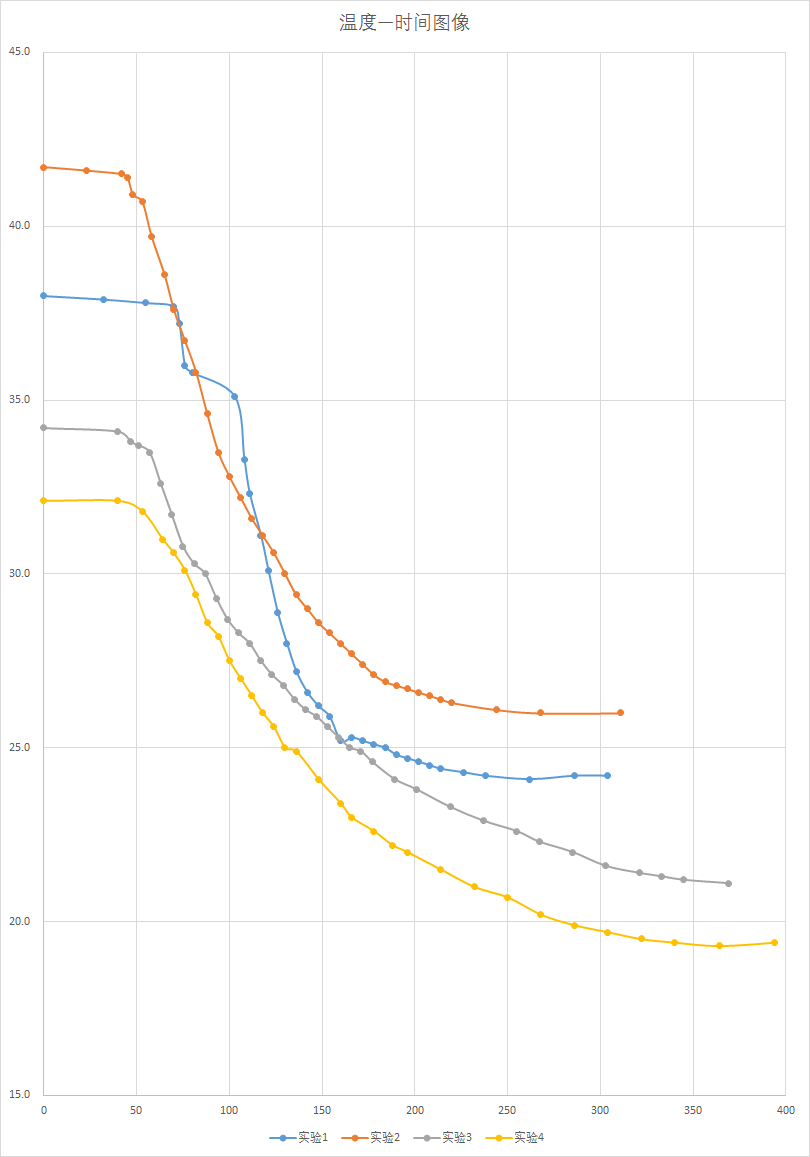
\includegraphics{fig.png}}
\caption{四次实验温度随时间变化的图线。}
\end{figure}


\end{document}
